\documentclass[a4paper,12pt]{article}

\usepackage{url}
\usepackage{epsfig}
\usepackage{graphics}
\usepackage{caption}
\usepackage{subcaption}
\usepackage{fancyhdr}
\usepackage{breakcites}
\usepackage[mode=buildnew]{standalone}% requires -shell-escape
\usepackage{tikz}
\usetikzlibrary{calc}
\usetikzlibrary{positioning}

\graphicspath{{pictures/}}

\title{Simultaneous Localization And Mapping in a domestic environment}
\author{\hspace*{-0.5cm}
\begin{tabular}{cccc}
Report Author &  Group Partner \\
Paul Rousse &  Jiaheng Qiu \\
\end{tabular}} 
\date{}

\pagestyle{fancy}
\fancyhf{}
\setlength{\headheight}{15pt}
\lhead{EL2320}
\rhead{\today}

\begin{document}

\maketitle
\thispagestyle{fancy}

\begin{abstract}

Many applications of mobile robots take place in a domestic environment (cleaning robot, wheelchair). Localization and mapping are the first needed knowledge in order that the robot can move in the area. Non professional applications can not benefit from high quality sensors. We tried to work with PSD infrared range sensor.
As in most domestical environments, the map can be drawn with lines (that stands for walls) that are either parallel either orthogonal.
An Extended Kalman Filter that estimate state with raw measures has been used, in this way we managed to avoid any heavy algorithm of line extraction.
We succefully implemented an algorithm that work on simulation.

\end{abstract}
\clearpage

\section{Introduction}
In most applications of mobile robot it is crucial to know the position of the robot in order to success in its task.
However, it is not always possible to get any previous knowledge about the environment where the robot evolve in.
That is what the SLAM problem tries to solve: localizate the robot while simultaneously building a map of the environment, and concurrently trying to minimize errors.
The Silmutaneous Localization And Mapping problem (SLAM) has been one of the most active field of research in robotic the last 3 decade.~\cite{Whyte06} sum up most of the work on SLAM.

Many different algorithms for SLAM have been developped, mainly because the outcomes of the algorithm depends on the sensors you have, the type of features of your map and the robot motion model.
The laser range finder meet a great success in the researcher community (\cite{jensfelt1999laser};\cite{diosi2005laser}) because of the quality of the measure: "null" propagation time and fairly good range and angular accuracy.
However the expensive cost of this sensor keep back costumer from any integration in any unprofessional mobile robot.
This explain the interest of researchers and companies in devlopping algorithm wich can works with cheaper sensors such as the sonar sensor (\cite{zunino2001simultaneous}; \cite{choi2008line}) or PSD infrared sensors (\cite{Abrate_experimentalekf-based}).

This challenge is mostly about how to build a SLAM algorithm with sparse and noisy data.
It is not always possible to take advantages of previous algorithm developped for laser range sensor because most of the time the number of sensors are much fewer than the number of measure of the laser scan.
Most of the work try to add constraints to the map in order to reduce the number of possibilities for the mapping and therefore to reduce the error of the map estimation. \cite{zunino2001simultaneous} use an algorithm that can take advantages of geometrics constraints of an indoor environment in order to perform the classification step with only a few and noisy data: \textit{Triangulation Based Fusion} (\cite{wijk1998triangulation}). This method let to perform a SLAM localization with point features which are defined as intersection of 2 lines features. In practice, points are detected in corner of a wall or a furniture.
However this method is relevant only when the roboot cross a corner. And therefore, the estimation does not take care of the distance of the robot from a straight wall.

\cite{choi2005robust} has taken advantage of both point features and line features by combining the TBF method and a line extraction algorithm. The feature extraction is used as a measure for the EKF implementation.
In \cite{choi2008line}, geometric constraints are used. Every measured point is stored and used in order to measure features of the map.
As for \cite{nguyen2006orthogonal}, geometric constraints (such as parallel and orthogonal walls) add information to the map generation and in this way it improve the estimation of localization and mapping.

\subsection{Contribution}
There are 3 main contributions in this article.
First an implementation of a SLAM algorithm with line-feature. Unlike point feature SLAM implementation, line feature have the disadvantages of being contiuous.
Second, we implemented a geometric constraint of parallel and orthogonal walls inside the EKF (instead of using a constrained line extraction).
Third, we manage to get ride of any heavy line extraction algorithm, and we show that a very simple algorithm can be used in order to create new features to the state vector.

\subsection{Outline}

The first section will present a review of the previous workk. The second, the implementation of our SLAM algorithm. And the third part will focus on results and limitation of our algorithm.

\section{Related work}
\label{sec:relwork}

Cost constraints have led researchers to developpe SLAM algorithm with sparse and noisy sensors.
Some solutions based on distance sensors has been proposed.
The main idea is to use furnitures as a map for the robot.

The first approach was to apply the same theory as for laser range sensor.
The idea was to use raw data to detect lines, then to extract lines and use it as a measure in the EKF.
If enough sensors was available, the line detection was be performed on incoming rax data at each step (\cite{grossmann2001robust}), if just a few are available, the line detection is performed on a set of points measured on several steps.

That is the strategy of \cite{choi2008line}, they made an implementation of the SLAM algorithm in an indoor environment by using a smart pre-treatment of all incoming measures from sonar sensors since the beginning of the mapping. This pre-treatment allow to reduce outlier generations and to perform an easier point-to-line association.
After this pre-treatment, line features are extracted thanks to a constrained Hough transform. The EKF estimate each line features independently.
Therefore the constrained is set inside the measure and not inside the EKF.

However, the Hough transform used in \cite{choi2008line} is not a probabilistic tool, it is an approximation of a probabilistic tool (\cite{stephens1991probabilistic}).
Therefore, they developpe their own covariance calculation which does not take in account the uncertainty on measure.
This empirical method make the EKF difficult to adjust (the uncartainty on the measure does not affect the empirical covariance computation on the Hough transform!

\section{My method}
\label{sec:method}

% Choix strategique
Most of the SLAM line-feature implemetation focus on measuring the line parameters in the EKF. We have choosen to directly use the measures of sonars.
% Algorithm general
This choice was made in order to avoid implementing any Hough transform that will take too much computational ressources.


\subsection{Extended Kalman Filter}
\label{sec:EKF}

First, we will present the EKF method without any geometric constraints.
The EKF model is the same as \cite{zunino2001simultaneous} for the predict step: the state of the EKF is represented by the state of the robot $\mathbf{x_r} = \left [x_r,y_r,\theta_r \right ]^T$ followed by the $N_f$ state vectors of features.
The $i^{th}$ feature is represented just by its parameters in polar coordinates, $\mathbf{x_i} = [\rho_i, \theta_i]^T$.

The predict step does not affect covariance matrices of features because they are not part of the dynamics (they are just measurements).

The observation model compute the distance from the sensor to the $i^{th}$ wall feature in direction of the sensor. $\psi$ is the angle of the sensor in the reference of the robot and $d$ the sensor position along the robot.

\begin{equation}
h_i(\mathbf{x}) =\frac{ x_r \: cos \, \theta_i + y_r \: sin \, \theta_i - \rho_i + d\: cos(\theta_r-\theta_i)}{cos(\theta_i-\theta_r-\psi)} 
\end{equation}

\begin{figure}[ht]
\centering
\begin{minipage}[b]{0.45\linewidth}

\centering
	\includestandalone[width=1.0\linewidth]{robot}
  	\caption{Robot parameters definitions. The robot (in blue) is performing one measure (in red) of the $i^{th}$ feature (in green).}
  	\label{fig:minipage1}
\end{minipage}
\quad
\begin{minipage}[b]{0.45\linewidth}
\centering
	\includestandalone[width=.8\linewidth]{algo}
  	\caption{Line extraction algorithm.}
\label{fig:minipage2}
\end{minipage}
\end{figure}
% Qu'est-ce-que ça fait là!!!
The computation of the jacobian show that the farer the distance measured is, higher is the uncertainty (because in this way the angle of the impacted measure is very low and the uncertainties on angles $\theta_r$ and $\theta_i$ have more influence).
Therefore if we want to have a precise estimation of the wall we should have orthogonal measures from it. The most optimal way to set sensors is to set them al around the robot.

\subsection{Geometric constraints}
\label{sec:geom}

Geometrics constraints are both represented in the feature addition process and in the state vector of the EKF.
We added a state variable $\alpha$ that represent the global orientation of the map according to the initial robot position.

%TODO shéma de la map et de alpha

The state vector of the EKF become:

\begin{equation}
\mathbf{X} = 
\left [
\begin{array}{ccccc}
\mathbf{x_r}&
\alpha& 
\mathbf{x_1}&
\cdots &  
\mathbf{x_{N_f}}
\end{array}
\right ]^T
\end{equation}

We compute the observation model with the geometric constraint:

\begin{equation}
h_i(\mathbf{x}) =\frac{ x_r \: cos \, \beta_i(\alpha) + y_r \: sin \, \beta_i(\alpha) - \rho_i + d\: cos(\theta_r-\beta_i(\alpha))}{cos(\beta_i(\alpha)-\theta_r-\psi)} 
\end{equation}

with:

\begin{equation}
\begin{array}{l}
\beta_i(\alpha) = \alpha - k \: \frac{\pi}{2}\\
\mathit{with } \: k = \left \lfloor (\alpha-\theta_i) \: \frac{2 }{\pi} +\frac{1}{2} \right \rfloor
\end{array}
\end{equation}

In other words, $\beta_i$ is the closest angle from $\theta_i$ which verify $\alpha \equiv \beta_i \left [ \frac{\pi}{2} \right ]$.

In order to compute the jacobian matrix, we set:

\begin{equation}
\frac{\partial h}{\partial \alpha} = \frac{\partial h}{\partial \theta_i}
\end{equation}

with $i$ the observed feature.

\subsection{Features addition}
\label{sec:features}

After each execution of the EKF step, outliers are saved in a buffer of a fixed size $N_{buffer}$.
This buffer is used then to perform the line feature extraction.

%\begin{figure}
%  	\centering
%\end{figure}

An unsupervised clustering algorithm is then used in order to seperat measures that do not come from the same wall. This 

First we try to detect if dataset is just noise or a line feature. We do this by comparing the covariance of the a cluster of points to the covariance of the uncertainty of these points. If the covariance is 
Then we can perform the line extraction step. We use the maximum of likelihood to choose if the new feature will be a vertical or an horizontal line. 

%TODO talk about sigma and finish explanation

% Sigma initialisation

\subsection{Implementation}

The clustering algorithm really depends on the number of sensors and how much the measures are noisy. If the measures are not so noisy and they are few sensors, then the classification can be performed just with indexes of the sensors (the measure is classified by the sensor it is coming from).
Otherwise a clustering algorithm is necessary: we used the DBSCAN discussed in \cite{ester1996density}. The DBSCAN algorithm classify in the same cluster points wich are closer than a given distance $\epsilon$.

This choice is not the optimal one, and we beleive that it is possible to choose a better one that take in account constraints and probability consideration (such as probability distribution parameters of the hit point after a measure).
However, as long as data are not so noisy, the DBSCAN algorithm is enough.

\section{Experimental results}
\label{sec:exps}

% Resultats sans beaucoup d'erreur
% afficher aussi courbe sigma d'une feature

\subsection{Analyse of the EKF behavior}
% EKF avec les features à l'initialisation
As shown in the figure \ref{fig:noerr}, the algorithm succefully manage to draw the map with line features and at the same time correct the trajectory. 
In this simulation, we gave a good and precise idea of $\alpha$. 

The unceartainty on features alway decrease (see figure \ref{fig:noerr_fi_sig}). This is a property of the EKF integration: during the predict step, because features do not take part in the dynamics (unlike the robot), the unceartainties do not increase. Since the update step always increases the belief of the state, the covariance matrix of the feature can just decrease.
This is a real issue in case of slidding motion of the robot: whatever the uncertainty $Q$ you have on the measure, the belief of the feature will increase. Therefore the EKF will always change the robot position because this is the only variable in the state vector that is not fully certain (contrary to every other features parameters).


\begin{figure*}
        \centering
        
        ~ %add desired spacing between images, e. g. ~, \quad, \qquad, \hfill etc.
          %(or a blank line to force the subfigure onto a new line)
          
        \begin{subfigure}[t]{0.45\textwidth}
                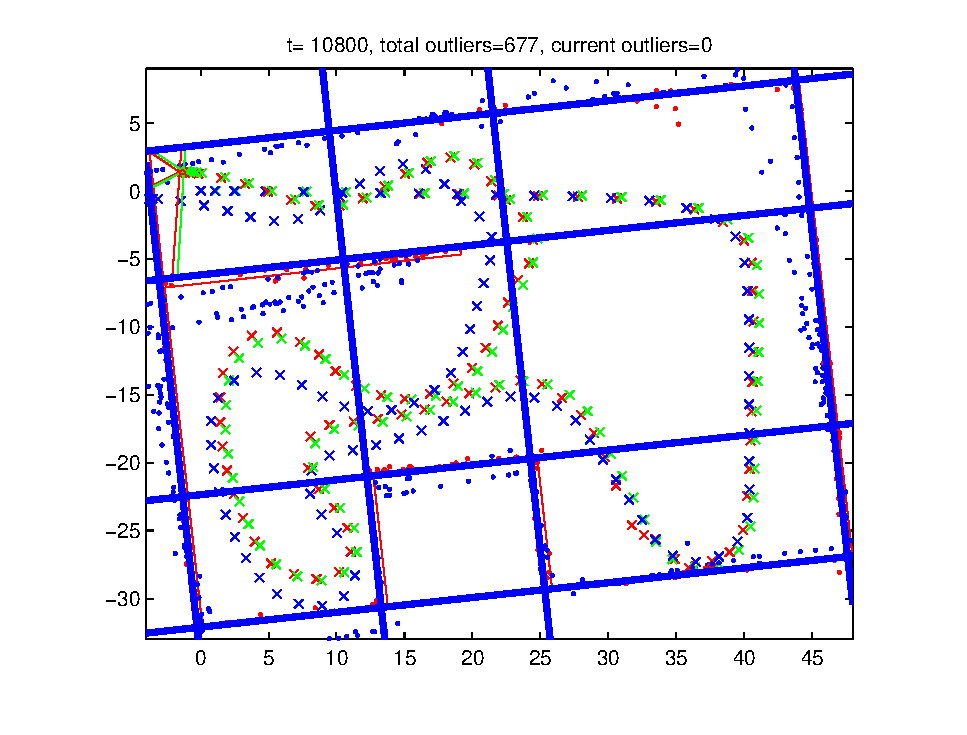
\includegraphics[width=\textwidth]{noerr_map2}
                \caption{Map of trajectories and features.}
                \label{fig:noerr_map}
        \end{subfigure}%
        \begin{subfigure}[t]{0.45\textwidth}
                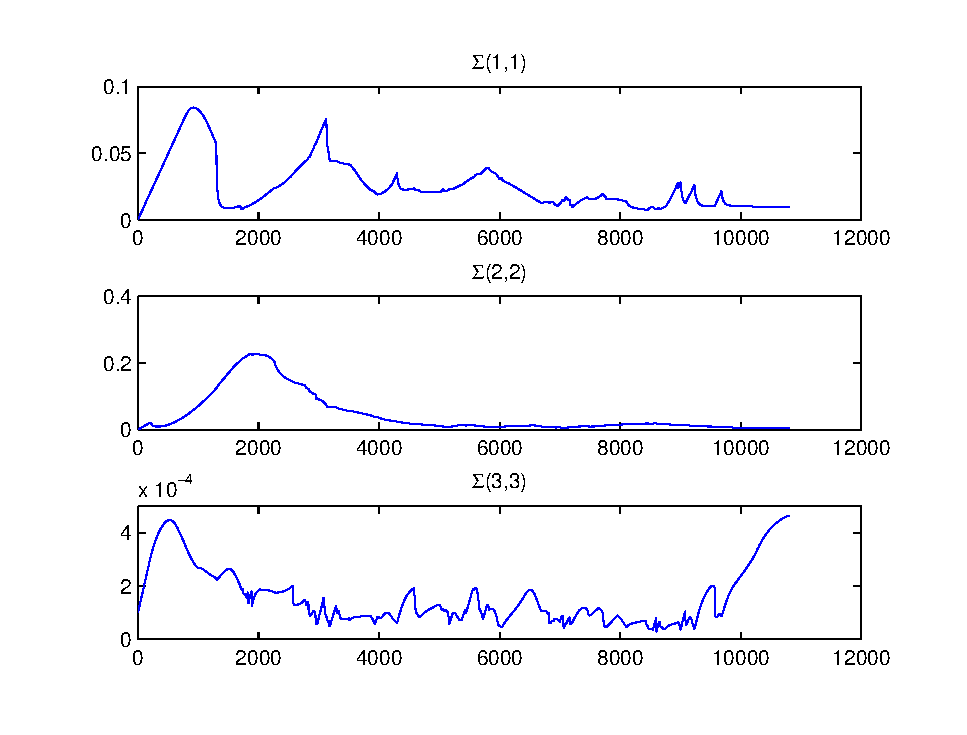
\includegraphics[width=\textwidth]{noerr_sig}
                \caption{Uncertainty of the measure of the estimated position.}
                \label{fig:noerr_sig}
        \end{subfigure}
        
        %% Feature figure
        \begin{subfigure}[t]{0.45\textwidth}
                \includegraphics[width=\textwidth]{noerr_f1_mu}
                \caption{Estimated parameters of the first feature.}
                \label{fig:noerr_fi_mu}
        \end{subfigure}
        \begin{subfigure}[t]{0.45\textwidth}
                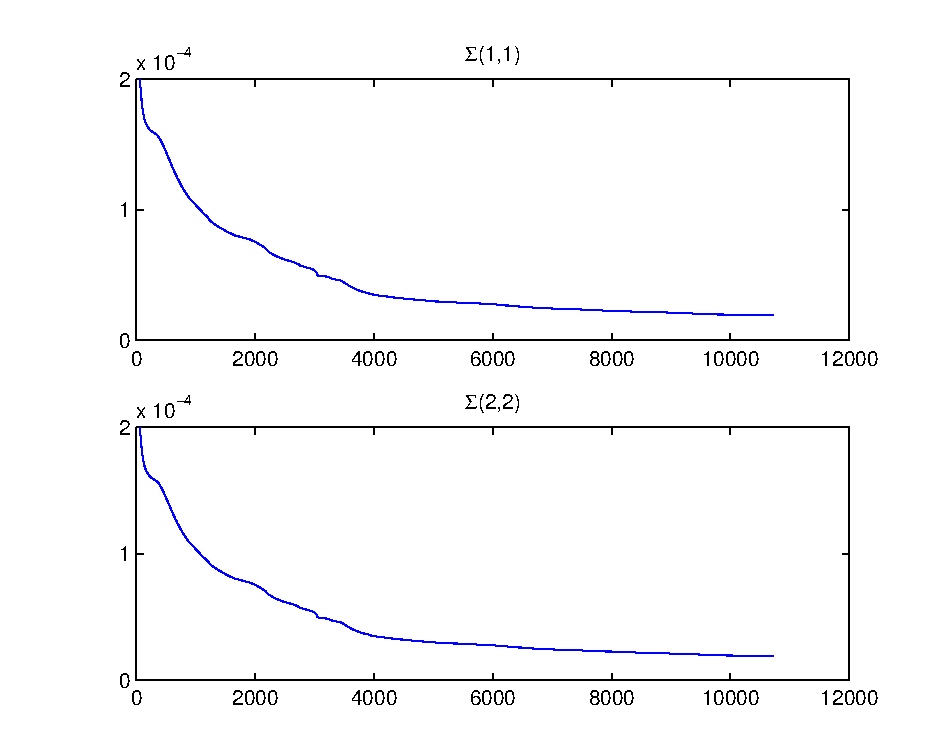
\includegraphics[width=\textwidth]{noerr_f1_sig}
                \caption{Coefficient values of the first feature covariance matrix.}
                \label{fig:noerr_fi_sig}
        \end{subfigure}
        
        \caption{Map (\ref{fig:noerr_map}) and sigma coefficients (\ref{fig:noerr_sig}) of a simulation with a low noise on odometry mesure and sensors (about $10^{-2}(m/s, rad/s and m)$). The estimate trajectory of the robot (red crosses) is corrected thanks to the map estimation (blue lines) and "stick" to the true trajectory of the robot (in green) instead of following the basic odometry estimate trajectory (blue crosses). Figures \ref{fig:noerr_fi_mu} and \ref{fig:noerr_fi_sig} are graphes from the first feature the robot added to its state.}
\label{fig:noerr}
\end{figure*}

\subsection{Line extraction}

The line extraction algorithm is tuned with 2 main parameters:
\begin{itemize}
	\item $N_{buffer}$ the size of the dataset buffer
	\item $\Sigma_{noise}$ the guessed covariance matrix of noise on the measure.
\end{itemize}
The success of the algorithm mainly depends if the second parameters. 

The first one have too be big enough in order to have more points that just noise: if $N_{buffer}$ is too low and measure too noisy, we will never detect a trend of line (but just a gaussian distribution of points). So to detect lines, we need to have enough data. In figure \ref{fig:noerr}, it seems that $N_{buffer} = 100$ was a reasonable value.
The draw back of this is that the computatinal cost increase as the noise on measure increase (in case of our implementation, the complexity of the DBSCAN algorithm is $\mathcal{O}(n\log{}n)$).

$\Sigma_{noise}$ is a threshold that avoid line extraction algorithm if data are not realevant. So, if the data are noisy, we need to set $\Sigma_{noise}$ to a larger value than if they are not.

% Analyse de l'algo de line extraction
% influence de chaques parametres

\subsection{Data association}

Unlike point feature, line feature are continuous, when crossing a corner, it is difficult to keep the data association correct (see figure \ref{fig:alpha_trouble}).
More over, our implementation of slam with line feature does assume avery wall as an infinit line! 
This create even more spaces where the robot fail to do the right data association.

Currently, this is the main obstacle to the well execution of the algorithm.
We will discuss in the conclusion the possible solutions in order to get over this difficulty.

\begin{figure*}

        \begin{subfigure}[t]{0.45\textwidth}
                \includegraphics[width=\textwidth]{alpha_trouble_map}
                \caption{Robot measuring the first corner of the map.}
        \end{subfigure}
        \quad
        \begin{subfigure}[t]{0.45\textwidth}
                \includegraphics[width=\textwidth]{alpha_trouble}
                \caption{Plot of $\alpha$.}
        \end{subfigure}
	\caption{Each arrow match to a timestep where the robot measure the distance in a corner. The wrong association of the measure to the feature avoid the good estimation of alpha.}
	\label{fig:alpha_trouble}
\end{figure*}


\section{Summary and Conclusions (0.5--1 page)}
\label{sec:summary}

Summarize what you have done and make sure that your highlight your
contributions. 
You should not introduce new results in the summary.
 Results should be introduced in the main sections above.
Here you can speculate on how these results could be extended, what would
happen in other settings or how the method could be used other domains
and how to continue with the research in the future.
In this section you can put statements that one cannot understand unless you have read
the paper which is not possible in the abstract for example. You do
not need to be as formal in this section.



\bibliographystyle{apalike}
\bibliography{refs}


\end{document}
